\shorthandoff{:!} %règle un problème de compatibilité avec babel
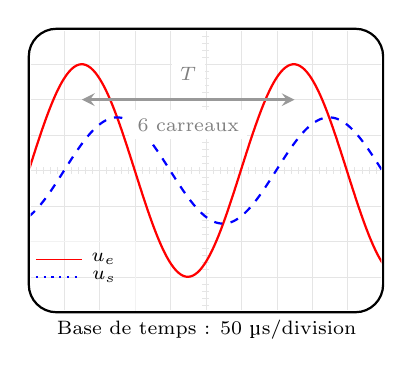
\begin{tikzpicture}[scale=0.45]
	%ecran oscilloscope
	\draw[black,thick,rounded corners=10pt] (0,0) rectangle (10,8) (0.5,-0.5) node[right]{\textcolor{Black}{\scriptsize{Base de temps : 50 µs/division}}}
	 ;
	\begin{scope} % permet d'appliquer des propriétés à une partie de code seulement
		\clip (0.05,0.05) rectangle (9.95,7.95);%créer une découpe de la fenêtre comme indiqué
		\foreach \x in {1,2,...,9}%Démarrage d'une boucle : "pour tout x appartenant à ..."
		{
			%la boucle est délimitée par une paire d'accolade
			\draw[gray!20, very thin] (\x,0.05) -- (\x,7.95);%thin = fin, il existe aussi very thin et ultra thin
		}
		\foreach \y in {1,2,...,7}
		{
			\draw[gray!20, very thin] (0.05,\y) -- (9.95,\y);
		}
		\foreach \x in {0.2,0.4,...,9.8}
		{
			\draw[gray!20, very thin] (\x,4.1) -- (\x,3.9);
		}
		\foreach \y in {0.2,0.4,...,7.8}
		{
			\draw [gray!20, very thin] (5.1,\y) -- (4.9,\y);
		}
		%FIN ecran oscilloscope
		% Les tensions d'entrée et de sortie
		\draw[yshift=4cm,color=red,thick,domain=0:10, smooth, samples=150] plot ({\x},{3*sin(1.05*\x r)});
		\draw[yshift=4cm,color=blue,dashed,thick,domain=0:10,smooth, samples=150] plot ({\x},{1.5*sin(1.05*\x r- pi/3 r)});
		%legende
		\draw [gray!10] (0,0) rectangle (3,2); %cadre
		\draw [red] (0.2,1.5)--(1.5,1.5) node [right] [red] {\textcolor{Black}{\scriptsize{$u_e$}}} ;
		\draw [blue, dotted, thick] (0.2,1)--(1.5,1) node [right] [blue] {\textcolor{Black}{\scriptsize{$u_s$}}};
		\draw[color=gray!80,line width=1pt,<->,>=stealth] (1.5,6) -- (7.5,6) node [midway, above] {\colorbox{white}{\textcolor{gray}{\scriptsize{$T$}}}} node [midway, below] {\colorbox{white}{\textcolor{gray}{\scriptsize{6 carreaux}}}} ;

		
	\end{scope}
\end{tikzpicture} 
\shorthandon{:!}